\section{Разбиения множеств}\label{sec:ch-1-sec-2}

\begin{definition}[Разбиение мн-в]
    Мн-во $A \neq \varnothing$, тогда семейство мн-в $K$ --- \definiendum{разбиение} $A$, если
    $\begin{cases}
         \bigcup K = A,\\
         \forall k, l \in K : k \neq l \imp k \cap l = \varnothing,\\
         \varnothing \notin K.
    \end{cases}$
\end{definition}

\begin{definition}[Измельчение разбиения]
    $\sqsupset K, L$ --- разбиения $A$, тогда говорят, что $K$ \definiendum{измельчает} $L$, если $\forall k \in K \imp \exists l \in L : k \subseteq l$.
\end{definition}

\begin{sh-remark}
    $\sqsupset K, L$ --- разбиения $A$, при этом $K$ измельчает $L$.
    Тогда будем говорить, что $K$ \definiendum{мельче} $L$, а $L$ \definiendum{крупнее} $K$.
\end{sh-remark}

\begin{definition}[Произведение разбиений]
    $\sqsupset K, L$ --- разбиения $A$, тогда \definiendum{произведение разбиений} --- самое крупное разбиение $A$, измельчающее $K$ и $L$.

    \begin{center}
        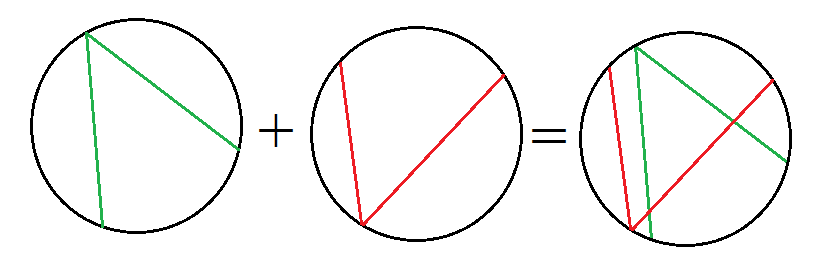
\includegraphics[scale=0.4]{res/произведение разбиений}
    \end{center}
\end{definition}

\begin{sh-proposition}
    Произведение разбиений существует.
\end{sh-proposition}

\begin{proof}
    Неформально: пересекаем все $X \in K$ со всеми $Y \in L$ и выкидываем пустые множества, получаем то, что надо.

    Чуть более формально: пусть $B = \set{ X \cap Y \mid X \in K, Y \in L, X \cap Y \neq \varnothing}$.

    $B$ --- разбиение $A$, так как $\forall b \in B \imp b \in \2{A}, b \neq \varnothing, \forall a \in A \imp \existu b \in B : a \in b$.

    Пусть $C$ --- тоже разбиение $A$, измельчающее $K$ и $L$, покажем, что $C$ измельчает и $B$.

    Пусть $c \in C \imp \exists X \in K\ \exists Y \in L : c \subseteq K$ и $c \subseteq L \imp c \subseteq K \cap L \imp \exists b = K \cap L \in B : c \subseteq b$.

    При желании можно накрутить ещё формализма, но так ли оно надо?
\end{proof}